\documentclass[1p]{elsarticle_modified}
%\bibliographystyle{elsarticle-num}

%\usepackage[colorlinks]{hyperref}
%\usepackage{abbrmath_seonhwa} %\Abb, \Ascr, \Acal ,\Abf, \Afrak
\usepackage{amsfonts}
\usepackage{amssymb}
\usepackage{amsmath}
\usepackage{amsthm}
\usepackage{scalefnt}
\usepackage{amsbsy}
\usepackage{kotex}
\usepackage{caption}
\usepackage{subfig}
\usepackage{color}
\usepackage{graphicx}
\usepackage{xcolor} %% white, black, red, green, blue, cyan, magenta, yellow
\usepackage{float}
\usepackage{setspace}
\usepackage{hyperref}

\usepackage{tikz}
\usetikzlibrary{arrows}

\usepackage{multirow}
\usepackage{array} % fixed length table
\usepackage{hhline}

%%%%%%%%%%%%%%%%%%%%%
\makeatletter
\renewcommand*\env@matrix[1][\arraystretch]{%
	\edef\arraystretch{#1}%
	\hskip -\arraycolsep
	\let\@ifnextchar\new@ifnextchar
	\array{*\c@MaxMatrixCols c}}
\makeatother %https://tex.stackexchange.com/questions/14071/how-can-i-increase-the-line-spacing-in-a-matrix
%%%%%%%%%%%%%%%

\usepackage[normalem]{ulem}

\newcommand{\msout}[1]{\ifmmode\text{\sout{\ensuremath{#1}}}\else\sout{#1}\fi}
%SOURCE: \msout is \stkout macro in https://tex.stackexchange.com/questions/20609/strikeout-in-math-mode

\newcommand{\cancel}[1]{
	\ifmmode
	{\color{red}\msout{#1}}
	\else
	{\color{red}\sout{#1}}
	\fi
}

\newcommand{\add}[1]{
	{\color{blue}\uwave{#1}}
}

\newcommand{\replace}[2]{
	\ifmmode
	{\color{red}\msout{#1}}{\color{blue}\uwave{#2}}
	\else
	{\color{red}\sout{#1}}{\color{blue}\uwave{#2}}
	\fi
}

\newcommand{\Sol}{\mathcal{S}} %segment
\newcommand{\D}{D} %diagram
\newcommand{\A}{\mathcal{A}} %arc


%%%%%%%%%%%%%%%%%%%%%%%%%%%%%5 test

\def\sl{\operatorname{\textup{SL}}(2,\Cbb)}
\def\psl{\operatorname{\textup{PSL}}(2,\Cbb)}
\def\quan{\mkern 1mu \triangleright \mkern 1mu}

\theoremstyle{definition}
\newtheorem{thm}{Theorem}[section]
\newtheorem{prop}[thm]{Proposition}
\newtheorem{lem}[thm]{Lemma}
\newtheorem{ques}[thm]{Question}
\newtheorem{cor}[thm]{Corollary}
\newtheorem{defn}[thm]{Definition}
\newtheorem{exam}[thm]{Example}
\newtheorem{rmk}[thm]{Remark}
\newtheorem{alg}[thm]{Algorithm}

\newcommand{\I}{\sqrt{-1}}
\begin{document}

%\begin{frontmatter}
%
%\title{Boundary parabolic representations of knots up to 8 crossings}
%
%%% Group authors per affiliation:
%\author{Yunhi Cho} 
%\address{Department of Mathematics, University of Seoul, Seoul, Korea}
%\ead{yhcho@uos.ac.kr}
%
%
%\author{Seonhwa Kim} %\fnref{s_kim}}
%\address{Center for Geometry and Physics, Institute for Basic Science, Pohang, 37673, Korea}
%\ead{ryeona17@ibs.re.kr}
%
%\author{Hyuk Kim}
%\address{Department of Mathematical Sciences, Seoul National University, Seoul 08826, Korea}
%\ead{hyukkim@snu.ac.kr}
%
%\author{Seokbeom Yoon}
%\address{Department of Mathematical Sciences, Seoul National University, Seoul, 08826,  Korea}
%\ead{sbyoon15@snu.ac.kr}
%
%\begin{abstract}
%We find all boundary parabolic representation of knots up to 8 crossings.
%
%\end{abstract}
%\begin{keyword}
%    \MSC[2010] 57M25 
%\end{keyword}
%
%\end{frontmatter}

%\linenumbers
%\tableofcontents
%
\newcommand\colored[1]{\textcolor{white}{\rule[-0.35ex]{0.8em}{1.4ex}}\kern-0.8em\color{red} #1}%
%\newcommand\colored[1]{\textcolor{white}{ #1}\kern-2.17ex	\textcolor{white}{ #1}\kern-1.81ex	\textcolor{white}{ #1}\kern-2.15ex\color{red}#1	}

{\Large $\underline{12n_{0320}~(K12n_{0320})}$}

\setlength{\tabcolsep}{10pt}
\renewcommand{\arraystretch}{1.6}
\vspace{1cm}\begin{tabular}{m{100pt}>{\centering\arraybackslash}m{274pt}}
\multirow{5}{120pt}{
	\centering
	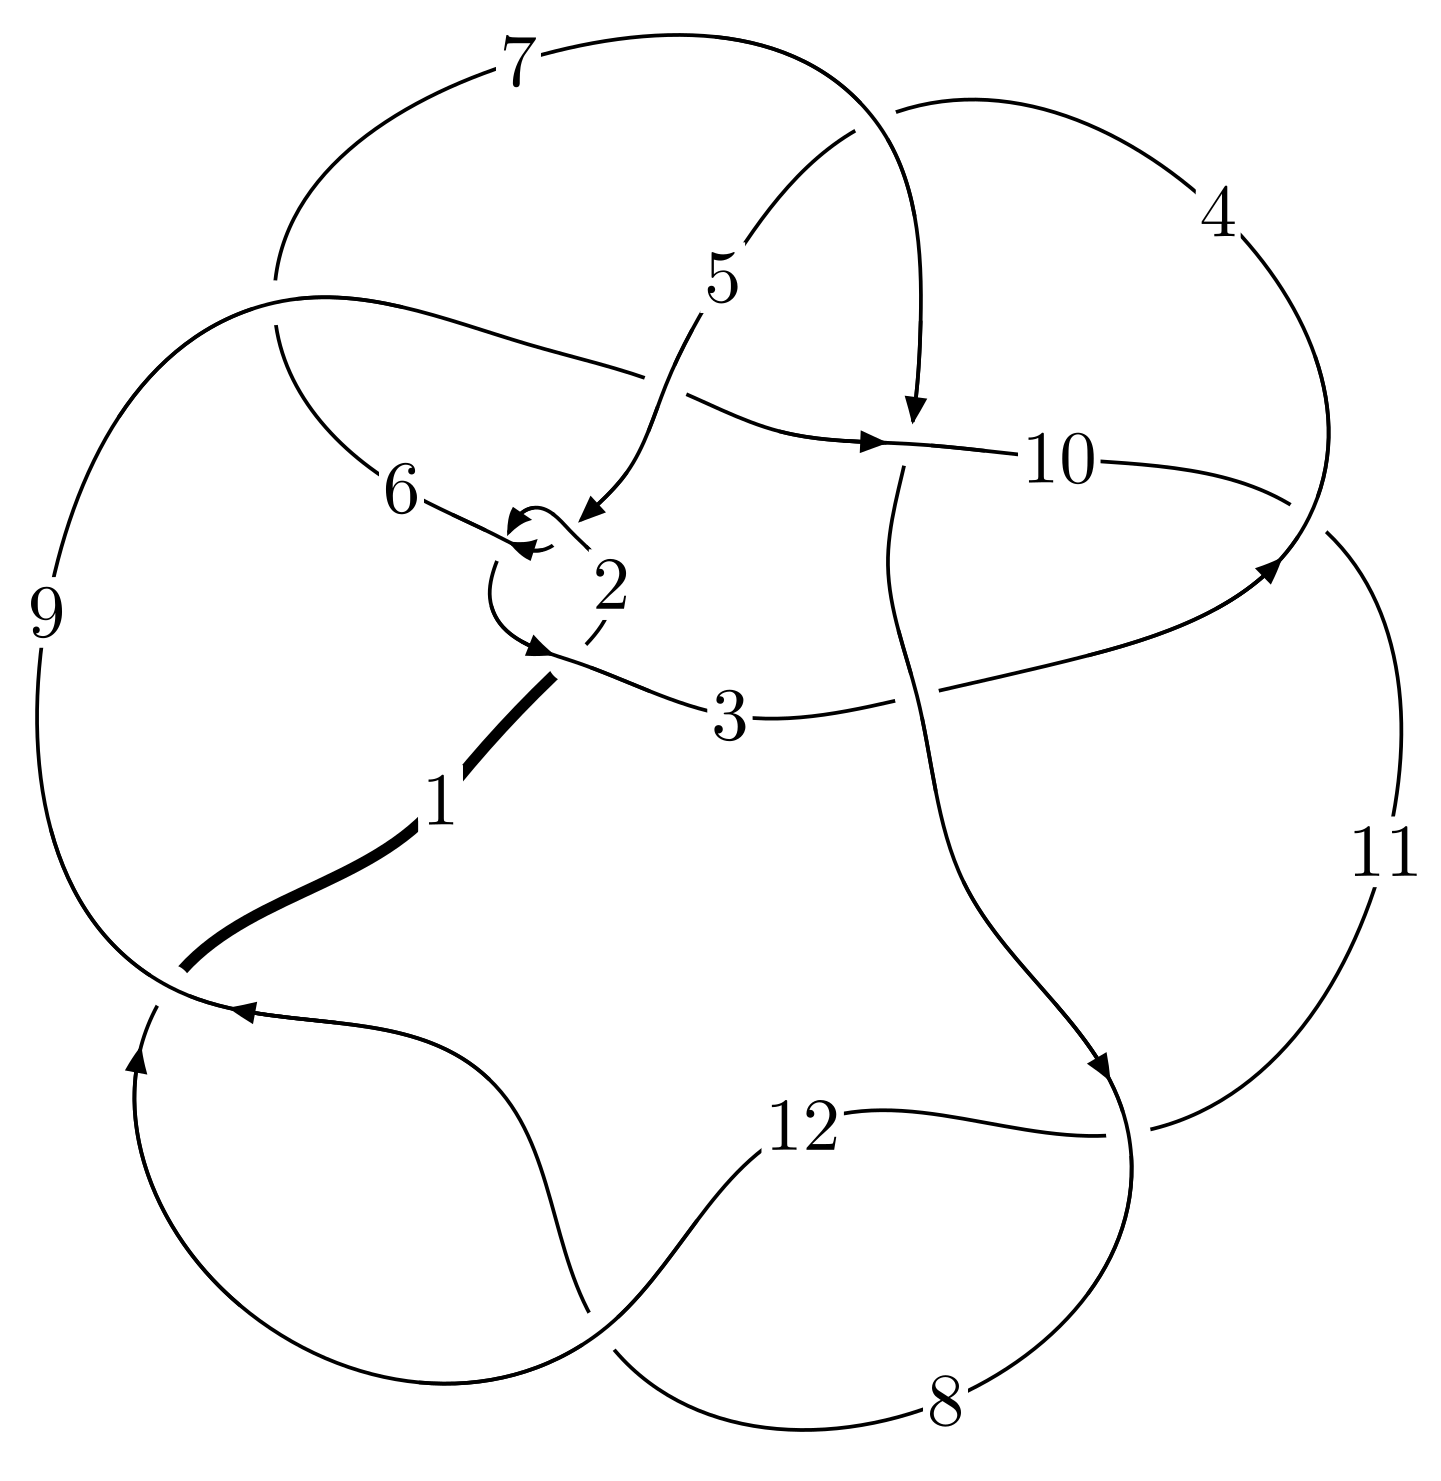
\includegraphics[width=112pt]{../../../GIT/diagram.site/Diagrams/png/2409_12n_0320.png}\\
\ \ \ A knot diagram\footnotemark}&
\allowdisplaybreaks
\textbf{Linearized knot diagam} \\
\cline{2-2}
 &
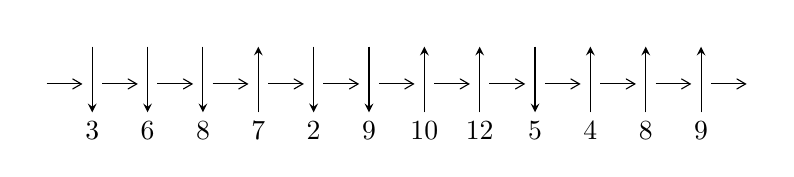
\begin{tikzpicture}[x=20pt, y=17pt]
	% nodes
	\node (C0) at (0, 0) {};
	\node (C1) at (1, 0) {};
	\node (C1U) at (1, +1) {};
	\node (C1D) at (1, -1) {3};

	\node (C2) at (2, 0) {};
	\node (C2U) at (2, +1) {};
	\node (C2D) at (2, -1) {6};

	\node (C3) at (3, 0) {};
	\node (C3U) at (3, +1) {};
	\node (C3D) at (3, -1) {8};

	\node (C4) at (4, 0) {};
	\node (C4U) at (4, +1) {};
	\node (C4D) at (4, -1) {7};

	\node (C5) at (5, 0) {};
	\node (C5U) at (5, +1) {};
	\node (C5D) at (5, -1) {2};

	\node (C6) at (6, 0) {};
	\node (C6U) at (6, +1) {};
	\node (C6D) at (6, -1) {9};

	\node (C7) at (7, 0) {};
	\node (C7U) at (7, +1) {};
	\node (C7D) at (7, -1) {10};

	\node (C8) at (8, 0) {};
	\node (C8U) at (8, +1) {};
	\node (C8D) at (8, -1) {12};

	\node (C9) at (9, 0) {};
	\node (C9U) at (9, +1) {};
	\node (C9D) at (9, -1) {5};

	\node (C10) at (10, 0) {};
	\node (C10U) at (10, +1) {};
	\node (C10D) at (10, -1) {4};

	\node (C11) at (11, 0) {};
	\node (C11U) at (11, +1) {};
	\node (C11D) at (11, -1) {8};

	\node (C12) at (12, 0) {};
	\node (C12U) at (12, +1) {};
	\node (C12D) at (12, -1) {9};
	\node (C13) at (13, 0) {};

	% arrows
	\draw[->,>={angle 60}]
	(C0) edge (C1) (C1) edge (C2) (C2) edge (C3) (C3) edge (C4) (C4) edge (C5) (C5) edge (C6) (C6) edge (C7) (C7) edge (C8) (C8) edge (C9) (C9) edge (C10) (C10) edge (C11) (C11) edge (C12) (C12) edge (C13) ;	\draw[->,>=stealth]
	(C1U) edge (C1D) (C2U) edge (C2D) (C3U) edge (C3D) (C4D) edge (C4U) (C5U) edge (C5D) (C6U) edge (C6D) (C7D) edge (C7U) (C8D) edge (C8U) (C9U) edge (C9D) (C10D) edge (C10U) (C11D) edge (C11U) (C12D) edge (C12U) ;
	\end{tikzpicture} \\
\hhline{~~} \\& 
\textbf{Solving Sequence} \\ \cline{2-2} 
 &
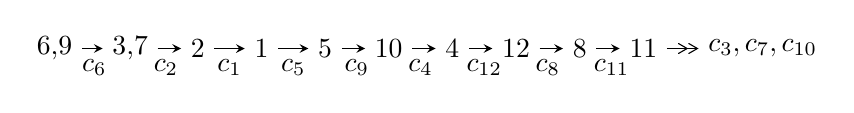
\begin{tikzpicture}[x=23pt, y=7pt]
	% node
	\node (A0) at (-1/8, 0) {6,9};
	\node (A1) at (17/16, 0) {3,7};
	\node (A2) at (17/8, 0) {2};
	\node (A3) at (25/8, 0) {1};
	\node (A4) at (33/8, 0) {5};
	\node (A5) at (41/8, 0) {10};
	\node (A6) at (49/8, 0) {4};
	\node (A7) at (57/8, 0) {12};
	\node (A8) at (65/8, 0) {8};
	\node (A9) at (73/8, 0) {11};
	\node (C1) at (1/2, -1) {$c_{6}$};
	\node (C2) at (13/8, -1) {$c_{2}$};
	\node (C3) at (21/8, -1) {$c_{1}$};
	\node (C4) at (29/8, -1) {$c_{5}$};
	\node (C5) at (37/8, -1) {$c_{9}$};
	\node (C6) at (45/8, -1) {$c_{4}$};
	\node (C7) at (53/8, -1) {$c_{12}$};
	\node (C8) at (61/8, -1) {$c_{8}$};
	\node (C9) at (69/8, -1) {$c_{11}$};
	\node (A10) at (11, 0) {$c_{3},c_{7},c_{10}$};

	% edge
	\draw[->,>=stealth]	
	(A0) edge (A1) (A1) edge (A2) (A2) edge (A3) (A3) edge (A4) (A4) edge (A5) (A5) edge (A6) (A6) edge (A7) (A7) edge (A8) (A8) edge (A9) ;
	\draw[->>,>={angle 60}]	
	(A9) edge (A10);
\end{tikzpicture} \\ 

\end{tabular} \\

\footnotetext{
The image of knot diagram is generated by the software ``\textbf{Draw programme}" developed by Andrew Bartholomew(\url{http://www.layer8.co.uk/maths/draw/index.htm\#Running-draw}), where we modified some parts for our purpose(\url{https://github.com/CATsTAILs/LinksPainter}).
}\phantom \\ \newline 
\centering \textbf{Ideals for irreducible components\footnotemark of $X_{\text{par}}$} 
 
\begin{align*}
I^u_{1}&=\langle 
1.94964\times10^{382} u^{72}+1.20690\times10^{383} u^{71}+\cdots+5.33896\times10^{384} b-1.10225\times10^{386},\\
\phantom{I^u_{1}}&\phantom{= \langle  }-1.84504\times10^{385} u^{72}-1.15557\times10^{386} u^{71}+\cdots+1.20981\times10^{387} a+8.26575\times10^{388},\\
\phantom{I^u_{1}}&\phantom{= \langle  }u^{73}+6 u^{72}+\cdots-18561 u+1133\rangle \\
I^u_{2}&=\langle 
-362677236 u^{12}+287880043 u^{11}+\cdots+2896442647 b+2924763966,\\
\phantom{I^u_{2}}&\phantom{= \langle  }-938151764 u^{12}-1358804549 u^{11}+\cdots+2896442647 a-4249866059,\\
\phantom{I^u_{2}}&\phantom{= \langle  }u^{13}+u^{11}+11 u^{10}+2 u^9+8 u^8+62 u^7-17 u^6+25 u^5-7 u^4-10 u^3+2 u^2+1\rangle \\
I^u_{3}&=\langle 
u^4+2 u^3- u^2+b-2 u,\;2 u^5+5 u^4-2 u^3-9 u^2+a+u+4,\;u^6+3 u^5-5 u^3- u^2+2 u+1\rangle \\
\\
\end{align*}
\raggedright * 3 irreducible components of $\dim_{\mathbb{C}}=0$, with total 92 representations.\\
\footnotetext{All coefficients of polynomials are rational numbers. But the coefficients are sometimes approximated in decimal forms when there is not enough margin.}
\newpage
\renewcommand{\arraystretch}{1}
\centering \section*{I. $I^u_{1}= \langle 1.95\times10^{382} u^{72}+1.21\times10^{383} u^{71}+\cdots+5.34\times10^{384} b-1.10\times10^{386},\;-1.85\times10^{385} u^{72}-1.16\times10^{386} u^{71}+\cdots+1.21\times10^{387} a+8.27\times10^{388},\;u^{73}+6 u^{72}+\cdots-18561 u+1133 \rangle$}
\flushleft \textbf{(i) Arc colorings}\\
\begin{tabular}{m{7pt} m{180pt} m{7pt} m{180pt} }
\flushright $a_{6}=$&$\begin{pmatrix}1\\0\end{pmatrix}$ \\
\flushright $a_{9}=$&$\begin{pmatrix}0\\u\end{pmatrix}$ \\
\flushright $a_{3}=$&$\begin{pmatrix}0.0152507 u^{72}+0.0955166 u^{71}+\cdots+844.480 u-68.3229\\-0.00365172 u^{72}-0.0226055 u^{71}+\cdots-241.555 u+20.6453\end{pmatrix}$ \\
\flushright $a_{7}=$&$\begin{pmatrix}1\\u^2\end{pmatrix}$ \\
\flushright $a_{2}=$&$\begin{pmatrix}0.0115990 u^{72}+0.0729111 u^{71}+\cdots+602.925 u-47.6775\\-0.00365172 u^{72}-0.0226055 u^{71}+\cdots-241.555 u+20.6453\end{pmatrix}$ \\
\flushright $a_{1}=$&$\begin{pmatrix}-0.0167624 u^{72}-0.103452 u^{71}+\cdots-1190.73 u+109.121\\0.00289105 u^{72}+0.0179807 u^{71}+\cdots+190.095 u-18.3749\end{pmatrix}$ \\
\flushright $a_{5}=$&$\begin{pmatrix}0.0184116 u^{72}+0.114807 u^{71}+\cdots+1089.39 u-91.6124\\-0.00601210 u^{72}-0.0371863 u^{71}+\cdots-388.300 u+34.2741\end{pmatrix}$ \\
\flushright $a_{10}=$&$\begin{pmatrix}-0.00271928 u^{72}-0.0151351 u^{71}+\cdots-390.211 u+41.7955\\0.00573011 u^{72}+0.0357021 u^{71}+\cdots+366.128 u-31.6795\end{pmatrix}$ \\
\flushright $a_{4}=$&$\begin{pmatrix}0.0255847 u^{72}+0.159203 u^{71}+\cdots+1537.33 u-130.800\\-0.00565886 u^{72}-0.0350883 u^{71}+\cdots-371.217 u+32.7353\end{pmatrix}$ \\
\flushright $a_{12}=$&$\begin{pmatrix}-0.0167624 u^{72}-0.103452 u^{71}+\cdots-1190.73 u+109.121\\0.00250121 u^{72}+0.0155056 u^{71}+\cdots+155.679 u-15.1148\end{pmatrix}$ \\
\flushright $a_{8}=$&$\begin{pmatrix}0.0117290 u^{72}+0.0727452 u^{71}+\cdots+719.230 u-62.4670\\-0.00246932 u^{72}-0.0152327 u^{71}+\cdots-178.421 u+16.4833\end{pmatrix}$ \\
\flushright $a_{11}=$&$\begin{pmatrix}-0.0182906 u^{72}-0.113075 u^{71}+\cdots-1255.70 u+113.788\\0.000808248 u^{72}+0.00493055 u^{71}+\cdots+38.6483 u-5.11399\end{pmatrix}$\\&\end{tabular}
\flushleft \textbf{(ii) Obstruction class $= -1$}\\~\\
\flushleft \textbf{(iii) Cusp Shapes $= 0.0291619 u^{72}+0.179368 u^{71}+\cdots+1994.61 u-181.670$}\\~\\
\newpage\renewcommand{\arraystretch}{1}
\flushleft \textbf{(iv) u-Polynomials at the component}\newline \\
\begin{tabular}{m{50pt}|m{274pt}}
Crossings & \hspace{64pt}u-Polynomials at each crossing \\
\hline $$\begin{aligned}c_{1}\end{aligned}$$&$\begin{aligned}
&u^{73}+40 u^{72}+\cdots+26772 u+121
\end{aligned}$\\
\hline $$\begin{aligned}c_{2},c_{5}\end{aligned}$$&$\begin{aligned}
&u^{73}+2 u^{72}+\cdots+146 u-11
\end{aligned}$\\
\hline $$\begin{aligned}c_{3}\end{aligned}$$&$\begin{aligned}
&u^{73}+3 u^{72}+\cdots+31 u-1
\end{aligned}$\\
\hline $$\begin{aligned}c_{4}\end{aligned}$$&$\begin{aligned}
&u^{73}+7 u^{72}+\cdots-96 u+64
\end{aligned}$\\
\hline $$\begin{aligned}c_{6}\end{aligned}$$&$\begin{aligned}
&u^{73}-6 u^{72}+\cdots-18561 u-1133
\end{aligned}$\\
\hline $$\begin{aligned}c_{7}\end{aligned}$$&$\begin{aligned}
&u^{73}-3 u^{72}+\cdots-12 u-1
\end{aligned}$\\
\hline $$\begin{aligned}c_{8},c_{11},c_{12}\end{aligned}$$&$\begin{aligned}
&u^{73}- u^{72}+\cdots-11 u-1
\end{aligned}$\\
\hline $$\begin{aligned}c_{9}\end{aligned}$$&$\begin{aligned}
&u^{73}- u^{72}+\cdots-11 u-19
\end{aligned}$\\
\hline $$\begin{aligned}c_{10}\end{aligned}$$&$\begin{aligned}
&u^{73}+3 u^{72}+\cdots-23 u-1
\end{aligned}$\\
\hline
\end{tabular}\\~\\
\newpage\renewcommand{\arraystretch}{1}
\flushleft \textbf{(v) Riley Polynomials at the component}\newline \\
\begin{tabular}{m{50pt}|m{274pt}}
Crossings & \hspace{64pt}Riley Polynomials at each crossing \\
\hline $$\begin{aligned}c_{1}\end{aligned}$$&$\begin{aligned}
&y^{73}-8 y^{72}+\cdots+632441220 y-14641
\end{aligned}$\\
\hline $$\begin{aligned}c_{2},c_{5}\end{aligned}$$&$\begin{aligned}
&y^{73}-40 y^{72}+\cdots+26772 y-121
\end{aligned}$\\
\hline $$\begin{aligned}c_{3}\end{aligned}$$&$\begin{aligned}
&y^{73}-71 y^{72}+\cdots-323 y-1
\end{aligned}$\\
\hline $$\begin{aligned}c_{4}\end{aligned}$$&$\begin{aligned}
&y^{73}+29 y^{72}+\cdots-1084416 y-4096
\end{aligned}$\\
\hline $$\begin{aligned}c_{6}\end{aligned}$$&$\begin{aligned}
&y^{73}-34 y^{72}+\cdots+64177063 y-1283689
\end{aligned}$\\
\hline $$\begin{aligned}c_{7}\end{aligned}$$&$\begin{aligned}
&y^{73}-19 y^{72}+\cdots+32 y-1
\end{aligned}$\\
\hline $$\begin{aligned}c_{8},c_{11},c_{12}\end{aligned}$$&$\begin{aligned}
&y^{73}-17 y^{72}+\cdots-37 y-1
\end{aligned}$\\
\hline $$\begin{aligned}c_{9}\end{aligned}$$&$\begin{aligned}
&y^{73}+21 y^{72}+\cdots-26327 y-361
\end{aligned}$\\
\hline $$\begin{aligned}c_{10}\end{aligned}$$&$\begin{aligned}
&y^{73}+53 y^{72}+\cdots+217 y-1
\end{aligned}$\\
\hline
\end{tabular}\\~\\
\newpage\flushleft \textbf{(vi) Complex Volumes and Cusp Shapes}
$$\begin{array}{c|c|c}  
\text{Solutions to }I^u_{1}& \I (\text{vol} + \sqrt{-1}CS) & \text{Cusp shape}\\
 \hline 
\begin{aligned}
u &= -1.031340 + 0.008433 I \\
a &= -0.069808 + 1.084620 I \\
b &= \phantom{-}1.375400 - 0.230767 I\end{aligned}
 & -8.53900 - 6.42718 I & \phantom{-0.000000 } 0 \\ \hline\begin{aligned}
u &= -1.031340 - 0.008433 I \\
a &= -0.069808 - 1.084620 I \\
b &= \phantom{-}1.375400 + 0.230767 I\end{aligned}
 & -8.53900 + 6.42718 I & \phantom{-0.000000 } 0 \\ \hline\begin{aligned}
u &= \phantom{-}1.016880 + 0.247438 I \\
a &= \phantom{-}0.18301 + 1.43687 I \\
b &= -1.134700 - 0.389357 I\end{aligned}
 & -3.48643 - 1.34087 I & \phantom{-0.000000 } 0 \\ \hline\begin{aligned}
u &= \phantom{-}1.016880 - 0.247438 I \\
a &= \phantom{-}0.18301 - 1.43687 I \\
b &= -1.134700 + 0.389357 I\end{aligned}
 & -3.48643 + 1.34087 I & \phantom{-0.000000 } 0 \\ \hline\begin{aligned}
u &= -0.698200 + 0.781658 I \\
a &= -0.086270 - 0.883147 I \\
b &= \phantom{-}0.143676 + 0.967502 I\end{aligned}
 & \phantom{-}2.76121 + 4.17164 I & \phantom{-0.000000 } 0 \\ \hline\begin{aligned}
u &= -0.698200 - 0.781658 I \\
a &= -0.086270 + 0.883147 I \\
b &= \phantom{-}0.143676 - 0.967502 I\end{aligned}
 & \phantom{-}2.76121 - 4.17164 I & \phantom{-0.000000 } 0 \\ \hline\begin{aligned}
u &= \phantom{-}0.923453 + 0.507277 I \\
a &= -0.711008 - 0.775964 I \\
b &= \phantom{-}0.052883 + 0.873653 I\end{aligned}
 & -3.09395 - 3.25435 I & \phantom{-0.000000 } 0 \\ \hline\begin{aligned}
u &= \phantom{-}0.923453 - 0.507277 I \\
a &= -0.711008 + 0.775964 I \\
b &= \phantom{-}0.052883 - 0.873653 I\end{aligned}
 & -3.09395 + 3.25435 I & \phantom{-0.000000 } 0 \\ \hline\begin{aligned}
u &= \phantom{-}0.320327 + 1.015200 I \\
a &= \phantom{-}0.345566 + 1.000120 I \\
b &= \phantom{-}0.139397 - 0.696765 I\end{aligned}
 & \phantom{-}1.29497 - 2.48132 I & \phantom{-0.000000 } 0 \\ \hline\begin{aligned}
u &= \phantom{-}0.320327 - 1.015200 I \\
a &= \phantom{-}0.345566 - 1.000120 I \\
b &= \phantom{-}0.139397 + 0.696765 I\end{aligned}
 & \phantom{-}1.29497 + 2.48132 I & \phantom{-0.000000 } 0\\
 \hline 
 \end{array}$$\newpage$$\begin{array}{c|c|c}  
\text{Solutions to }I^u_{1}& \I (\text{vol} + \sqrt{-1}CS) & \text{Cusp shape}\\
 \hline 
\begin{aligned}
u &= -0.102722 + 0.909943 I \\
a &= \phantom{-}1.58395 - 1.09523 I \\
b &= -0.999021 + 0.236970 I\end{aligned}
 & -0.52366 + 1.44354 I & \phantom{-0.000000 } 0 \\ \hline\begin{aligned}
u &= -0.102722 - 0.909943 I \\
a &= \phantom{-}1.58395 + 1.09523 I \\
b &= -0.999021 - 0.236970 I\end{aligned}
 & -0.52366 - 1.44354 I & \phantom{-0.000000 } 0 \\ \hline\begin{aligned}
u &= -1.080410 + 0.103383 I \\
a &= -0.551852 + 0.897401 I \\
b &= -0.020100 - 0.900171 I\end{aligned}
 & -4.24460 - 3.95976 I & \phantom{-0.000000 } 0 \\ \hline\begin{aligned}
u &= -1.080410 - 0.103383 I \\
a &= -0.551852 - 0.897401 I \\
b &= -0.020100 + 0.900171 I\end{aligned}
 & -4.24460 + 3.95976 I & \phantom{-0.000000 } 0 \\ \hline\begin{aligned}
u &= -0.972563 + 0.495097 I \\
a &= -0.18790 + 1.67102 I \\
b &= \phantom{-}1.258500 - 0.462677 I\end{aligned}
 & -8.13571 + 8.75720 I & \phantom{-0.000000 } 0 \\ \hline\begin{aligned}
u &= -0.972563 - 0.495097 I \\
a &= -0.18790 - 1.67102 I \\
b &= \phantom{-}1.258500 + 0.462677 I\end{aligned}
 & -8.13571 - 8.75720 I & \phantom{-0.000000 } 0 \\ \hline\begin{aligned}
u &= \phantom{-}0.845098 + 0.817919 I \\
a &= \phantom{-}0.223034 + 0.772508 I \\
b &= \phantom{-}0.195678 - 0.647035 I\end{aligned}
 & \phantom{-}0.02539 - 2.06580 I & \phantom{-0.000000 } 0 \\ \hline\begin{aligned}
u &= \phantom{-}0.845098 - 0.817919 I \\
a &= \phantom{-}0.223034 - 0.772508 I \\
b &= \phantom{-}0.195678 + 0.647035 I\end{aligned}
 & \phantom{-}0.02539 + 2.06580 I & \phantom{-0.000000 } 0 \\ \hline\begin{aligned}
u &= \phantom{-}0.704242 + 0.317833 I \\
a &= -0.59265 - 2.07838 I \\
b &= \phantom{-}1.251460 + 0.483613 I\end{aligned}
 & -6.73334 - 1.65613 I & -2.92629 + 0.79234 I \\ \hline\begin{aligned}
u &= \phantom{-}0.704242 - 0.317833 I \\
a &= -0.59265 + 2.07838 I \\
b &= \phantom{-}1.251460 - 0.483613 I\end{aligned}
 & -6.73334 + 1.65613 I & -2.92629 - 0.79234 I\\
 \hline 
 \end{array}$$\newpage$$\begin{array}{c|c|c}  
\text{Solutions to }I^u_{1}& \I (\text{vol} + \sqrt{-1}CS) & \text{Cusp shape}\\
 \hline 
\begin{aligned}
u &= \phantom{-}0.556762 + 0.475035 I \\
a &= \phantom{-}0.324680 + 0.714527 I \\
b &= -1.215180 - 0.518061 I\end{aligned}
 & -1.72177 - 1.34235 I & \phantom{-}1.77903 + 5.54028 I \\ \hline\begin{aligned}
u &= \phantom{-}0.556762 - 0.475035 I \\
a &= \phantom{-}0.324680 - 0.714527 I \\
b &= -1.215180 + 0.518061 I\end{aligned}
 & -1.72177 + 1.34235 I & \phantom{-}1.77903 - 5.54028 I \\ \hline\begin{aligned}
u &= -0.457882 + 1.231170 I \\
a &= -0.082528 - 0.200066 I \\
b &= \phantom{-}0.705147 + 0.340560 I\end{aligned}
 & \phantom{-}1.30339 - 1.96383 I & \phantom{-0.000000 } 0 \\ \hline\begin{aligned}
u &= -0.457882 - 1.231170 I \\
a &= -0.082528 + 0.200066 I \\
b &= \phantom{-}0.705147 - 0.340560 I\end{aligned}
 & \phantom{-}1.30339 + 1.96383 I & \phantom{-0.000000 } 0 \\ \hline\begin{aligned}
u &= \phantom{-}1.327210 + 0.201548 I \\
a &= -0.032088 - 0.895329 I \\
b &= \phantom{-}1.295440 + 0.256609 I\end{aligned}
 & -9.63449 - 0.84683 I & \phantom{-0.000000 } 0 \\ \hline\begin{aligned}
u &= \phantom{-}1.327210 - 0.201548 I \\
a &= -0.032088 + 0.895329 I \\
b &= \phantom{-}1.295440 - 0.256609 I\end{aligned}
 & -9.63449 + 0.84683 I & \phantom{-0.000000 } 0 \\ \hline\begin{aligned}
u &= \phantom{-}1.279340 + 0.555895 I \\
a &= \phantom{-}0.041703 - 1.054370 I \\
b &= -0.324932 + 0.913616 I\end{aligned}
 & -4.31900 - 2.85477 I & \phantom{-0.000000 } 0 \\ \hline\begin{aligned}
u &= \phantom{-}1.279340 - 0.555895 I \\
a &= \phantom{-}0.041703 + 1.054370 I \\
b &= -0.324932 - 0.913616 I\end{aligned}
 & -4.31900 + 2.85477 I & \phantom{-0.000000 } 0 \\ \hline\begin{aligned}
u &= -1.293390 + 0.552574 I \\
a &= \phantom{-}0.307125 - 0.021259 I \\
b &= \phantom{-}0.769443 + 0.511761 I\end{aligned}
 & \phantom{-}3.52478 - 2.09880 I & \phantom{-0.000000 } 0 \\ \hline\begin{aligned}
u &= -1.293390 - 0.552574 I \\
a &= \phantom{-}0.307125 + 0.021259 I \\
b &= \phantom{-}0.769443 - 0.511761 I\end{aligned}
 & \phantom{-}3.52478 + 2.09880 I & \phantom{-0.000000 } 0\\
 \hline 
 \end{array}$$\newpage$$\begin{array}{c|c|c}  
\text{Solutions to }I^u_{1}& \I (\text{vol} + \sqrt{-1}CS) & \text{Cusp shape}\\
 \hline 
\begin{aligned}
u &= -0.564547\phantom{ +0.000000I} \\
a &= \phantom{-}1.46692\phantom{ +0.000000I} \\
b &= \phantom{-}0.0693710\phantom{ +0.000000I}\end{aligned}
 & \phantom{-}1.42881\phantom{ +0.000000I} & \phantom{-}7.52280\phantom{ +0.000000I} \\ \hline\begin{aligned}
u &= -1.19035 + 0.80455 I \\
a &= -0.040182 + 1.009980 I \\
b &= -0.285323 - 1.026970 I\end{aligned}
 & -2.73397 + 10.71610 I & \phantom{-0.000000 } 0 \\ \hline\begin{aligned}
u &= -1.19035 - 0.80455 I \\
a &= -0.040182 - 1.009980 I \\
b &= -0.285323 + 1.026970 I\end{aligned}
 & -2.73397 - 10.71610 I & \phantom{-0.000000 } 0 \\ \hline\begin{aligned}
u &= \phantom{-}0.82644 + 1.17623 I \\
a &= \phantom{-}0.666106 - 1.183330 I \\
b &= \phantom{-}0.932325 + 0.388293 I\end{aligned}
 & -0.79582 - 6.86751 I & \phantom{-0.000000 } 0 \\ \hline\begin{aligned}
u &= \phantom{-}0.82644 - 1.17623 I \\
a &= \phantom{-}0.666106 + 1.183330 I \\
b &= \phantom{-}0.932325 - 0.388293 I\end{aligned}
 & -0.79582 + 6.86751 I & \phantom{-0.000000 } 0 \\ \hline\begin{aligned}
u &= -0.529293 + 0.181821 I \\
a &= -0.639919 - 1.224910 I \\
b &= -1.275540 + 0.261362 I\end{aligned}
 & -2.37007 + 0.33063 I & -5.36190 + 8.76599 I \\ \hline\begin{aligned}
u &= -0.529293 - 0.181821 I \\
a &= -0.639919 + 1.224910 I \\
b &= -1.275540 - 0.261362 I\end{aligned}
 & -2.37007 - 0.33063 I & -5.36190 - 8.76599 I \\ \hline\begin{aligned}
u &= -1.42533 + 0.24670 I \\
a &= \phantom{-}0.050785 - 0.805780 I \\
b &= \phantom{-}0.891619 + 0.767472 I\end{aligned}
 & \phantom{-}3.06820 - 2.89868 I & \phantom{-0.000000 } 0 \\ \hline\begin{aligned}
u &= -1.42533 - 0.24670 I \\
a &= \phantom{-}0.050785 + 0.805780 I \\
b &= \phantom{-}0.891619 - 0.767472 I\end{aligned}
 & \phantom{-}3.06820 + 2.89868 I & \phantom{-0.000000 } 0 \\ \hline\begin{aligned}
u &= -1.19516 + 0.92757 I \\
a &= \phantom{-}0.115452 + 1.011240 I \\
b &= \phantom{-}1.249180 - 0.552747 I\end{aligned}
 & -0.61277 + 9.60861 I & \phantom{-0.000000 } 0\\
 \hline 
 \end{array}$$\newpage$$\begin{array}{c|c|c}  
\text{Solutions to }I^u_{1}& \I (\text{vol} + \sqrt{-1}CS) & \text{Cusp shape}\\
 \hline 
\begin{aligned}
u &= -1.19516 - 0.92757 I \\
a &= \phantom{-}0.115452 - 1.011240 I \\
b &= \phantom{-}1.249180 + 0.552747 I\end{aligned}
 & -0.61277 - 9.60861 I & \phantom{-0.000000 } 0 \\ \hline\begin{aligned}
u &= -1.40807 + 0.66939 I \\
a &= \phantom{-}0.460393 + 0.498489 I \\
b &= \phantom{-}0.913659 - 0.284641 I\end{aligned}
 & \phantom{-}0.829050 + 0.928279 I & \phantom{-0.000000 } 0 \\ \hline\begin{aligned}
u &= -1.40807 - 0.66939 I \\
a &= \phantom{-}0.460393 - 0.498489 I \\
b &= \phantom{-}0.913659 + 0.284641 I\end{aligned}
 & \phantom{-}0.829050 - 0.928279 I & \phantom{-0.000000 } 0 \\ \hline\begin{aligned}
u &= -0.37186 + 1.51517 I \\
a &= -0.603407 - 0.886155 I \\
b &= -0.791457 + 0.373687 I\end{aligned}
 & -0.66969 - 3.07517 I & \phantom{-0.000000 } 0 \\ \hline\begin{aligned}
u &= -0.37186 - 1.51517 I \\
a &= -0.603407 + 0.886155 I \\
b &= -0.791457 - 0.373687 I\end{aligned}
 & -0.66969 + 3.07517 I & \phantom{-0.000000 } 0 \\ \hline\begin{aligned}
u &= \phantom{-}0.168757 + 0.338708 I \\
a &= -1.39461 - 1.59302 I \\
b &= \phantom{-}0.849357 - 0.685739 I\end{aligned}
 & \phantom{-}7.96391 + 2.63534 I & \phantom{-}10.53738 - 3.36691 I \\ \hline\begin{aligned}
u &= \phantom{-}0.168757 - 0.338708 I \\
a &= -1.39461 + 1.59302 I \\
b &= \phantom{-}0.849357 + 0.685739 I\end{aligned}
 & \phantom{-}7.96391 - 2.63534 I & \phantom{-}10.53738 + 3.36691 I \\ \hline\begin{aligned}
u &= -1.60775 + 0.25073 I \\
a &= -0.058800 - 0.535382 I \\
b &= -1.270170 + 0.471642 I\end{aligned}
 & -8.07804 + 0.96725 I & \phantom{-0.000000 } 0 \\ \hline\begin{aligned}
u &= -1.60775 - 0.25073 I \\
a &= -0.058800 + 0.535382 I \\
b &= -1.270170 - 0.471642 I\end{aligned}
 & -8.07804 - 0.96725 I & \phantom{-0.000000 } 0 \\ \hline\begin{aligned}
u &= -1.62701 + 0.14118 I \\
a &= \phantom{-}0.057887 + 1.157310 I \\
b &= -0.885594 - 0.751718 I\end{aligned}
 & \phantom{-}4.19772 - 2.84969 I & \phantom{-0.000000 } 0\\
 \hline 
 \end{array}$$\newpage$$\begin{array}{c|c|c}  
\text{Solutions to }I^u_{1}& \I (\text{vol} + \sqrt{-1}CS) & \text{Cusp shape}\\
 \hline 
\begin{aligned}
u &= -1.62701 - 0.14118 I \\
a &= \phantom{-}0.057887 - 1.157310 I \\
b &= -0.885594 + 0.751718 I\end{aligned}
 & \phantom{-}4.19772 + 2.84969 I & \phantom{-0.000000 } 0 \\ \hline\begin{aligned}
u &= \phantom{-}0.332878 + 0.028795 I \\
a &= -6.64477 + 4.14556 I \\
b &= -0.856356 + 0.076377 I\end{aligned}
 & \phantom{-}0.469074 + 0.132162 I & -52.8630 - 35.7017 I \\ \hline\begin{aligned}
u &= \phantom{-}0.332878 - 0.028795 I \\
a &= -6.64477 - 4.14556 I \\
b &= -0.856356 - 0.076377 I\end{aligned}
 & \phantom{-}0.469074 - 0.132162 I & -52.8630 + 35.7017 I \\ \hline\begin{aligned}
u &= \phantom{-}0.61123 + 1.63936 I \\
a &= -0.364083 + 0.786880 I \\
b &= \phantom{-}0.676939 - 0.447545 I\end{aligned}
 & \phantom{-}0.01496 - 3.34458 I & \phantom{-0.000000 } 0 \\ \hline\begin{aligned}
u &= \phantom{-}0.61123 - 1.63936 I \\
a &= -0.364083 - 0.786880 I \\
b &= \phantom{-}0.676939 + 0.447545 I\end{aligned}
 & \phantom{-}0.01496 + 3.34458 I & \phantom{-0.000000 } 0 \\ \hline\begin{aligned}
u &= \phantom{-}0.077199 + 0.194945 I \\
a &= -1.045320 + 0.356695 I \\
b &= -0.680238 + 1.054680 I\end{aligned}
 & \phantom{-}0.55649 + 4.84325 I & -9.6053 - 10.7522 I \\ \hline\begin{aligned}
u &= \phantom{-}0.077199 - 0.194945 I \\
a &= -1.045320 - 0.356695 I \\
b &= -0.680238 - 1.054680 I\end{aligned}
 & \phantom{-}0.55649 - 4.84325 I & -9.6053 + 10.7522 I \\ \hline\begin{aligned}
u &= \phantom{-}0.190020 + 0.008741 I \\
a &= \phantom{-}3.18173 + 0.88298 I \\
b &= -0.832237 - 0.401743 I\end{aligned}
 & -1.68584 - 0.75262 I & -4.20696 + 3.02462 I \\ \hline\begin{aligned}
u &= \phantom{-}0.190020 - 0.008741 I \\
a &= \phantom{-}3.18173 - 0.88298 I \\
b &= -0.832237 + 0.401743 I\end{aligned}
 & -1.68584 + 0.75262 I & -4.20696 - 3.02462 I \\ \hline\begin{aligned}
u &= \phantom{-}1.14874 + 1.41502 I \\
a &= -0.090176 - 0.812042 I \\
b &= \phantom{-}1.172430 + 0.484972 I\end{aligned}
 & -1.69151 - 6.95731 I & \phantom{-0.000000 } 0\\
 \hline 
 \end{array}$$\newpage$$\begin{array}{c|c|c}  
\text{Solutions to }I^u_{1}& \I (\text{vol} + \sqrt{-1}CS) & \text{Cusp shape}\\
 \hline 
\begin{aligned}
u &= \phantom{-}1.14874 - 1.41502 I \\
a &= -0.090176 + 0.812042 I \\
b &= \phantom{-}1.172430 - 0.484972 I\end{aligned}
 & -1.69151 + 6.95731 I & \phantom{-0.000000 } 0 \\ \hline\begin{aligned}
u &= -1.72102 + 0.61105 I \\
a &= -0.084879 - 0.409811 I \\
b &= -0.915829 - 0.198212 I\end{aligned}
 & \phantom{-}4.61519 - 0.89594 I & \phantom{-0.000000 } 0 \\ \hline\begin{aligned}
u &= -1.72102 - 0.61105 I \\
a &= -0.084879 + 0.409811 I \\
b &= -0.915829 + 0.198212 I\end{aligned}
 & \phantom{-}4.61519 + 0.89594 I & \phantom{-0.000000 } 0 \\ \hline\begin{aligned}
u &= \phantom{-}1.69805 + 0.77805 I \\
a &= \phantom{-}0.034519 + 1.038170 I \\
b &= -1.197940 - 0.626774 I\end{aligned}
 & -6.94494 - 8.52178 I & \phantom{-0.000000 } 0 \\ \hline\begin{aligned}
u &= \phantom{-}1.69805 - 0.77805 I \\
a &= \phantom{-}0.034519 - 1.038170 I \\
b &= -1.197940 + 0.626774 I\end{aligned}
 & -6.94494 + 8.52178 I & \phantom{-0.000000 } 0 \\ \hline\begin{aligned}
u &= \phantom{-}1.78485 + 0.62481 I \\
a &= -0.035007 + 0.478103 I \\
b &= -1.246140 - 0.443705 I\end{aligned}
 & -7.01799 - 7.84696 I & \phantom{-0.000000 } 0 \\ \hline\begin{aligned}
u &= \phantom{-}1.78485 - 0.62481 I \\
a &= -0.035007 - 0.478103 I \\
b &= -1.246140 + 0.443705 I\end{aligned}
 & -7.01799 + 7.84696 I & \phantom{-0.000000 } 0 \\ \hline\begin{aligned}
u &= -1.64823 + 1.00779 I \\
a &= \phantom{-}0.019327 - 0.971347 I \\
b &= -1.246010 + 0.626078 I\end{aligned}
 & -5.7190 + 16.6662 I & \phantom{-0.000000 } 0 \\ \hline\begin{aligned}
u &= -1.64823 - 1.00779 I \\
a &= \phantom{-}0.019327 + 0.971347 I \\
b &= -1.246010 - 0.626078 I\end{aligned}
 & -5.7190 - 16.6662 I & \phantom{-0.000000 } 0 \\ \hline\begin{aligned}
u &= \phantom{-}1.64963 + 1.05225 I \\
a &= \phantom{-}0.079258 - 0.840196 I \\
b &= \phantom{-}1.137360 + 0.514079 I\end{aligned}
 & -2.59231 - 6.57079 I & \phantom{-0.000000 } 0\\
 \hline 
 \end{array}$$\newpage$$\begin{array}{c|c|c}  
\text{Solutions to }I^u_{1}& \I (\text{vol} + \sqrt{-1}CS) & \text{Cusp shape}\\
 \hline 
\begin{aligned}
u &= \phantom{-}1.64963 - 1.05225 I \\
a &= \phantom{-}0.079258 + 0.840196 I \\
b &= \phantom{-}1.137360 - 0.514079 I\end{aligned}
 & -2.59231 + 6.57079 I & \phantom{-0.000000 } 0 \\ \hline\begin{aligned}
u &= \phantom{-}0.18175 + 2.19918 I \\
a &= \phantom{-}0.299156 + 0.533354 I \\
b &= -0.867813 - 0.323965 I\end{aligned}
 & -0.85745 - 6.14484 I & \phantom{-0.000000 } 0 \\ \hline\begin{aligned}
u &= \phantom{-}0.18175 - 2.19918 I \\
a &= \phantom{-}0.299156 - 0.533354 I \\
b &= -0.867813 + 0.323965 I\end{aligned}
 & -0.85745 + 6.14484 I & \phantom{-0.000000 } 0\\
 \hline 
 \end{array}$$\newpage\newpage\renewcommand{\arraystretch}{1}
\centering \section*{II. $I^u_{2}= \langle -3.63\times10^{8} u^{12}+2.88\times10^{8} u^{11}+\cdots+2.90\times10^{9} b+2.92\times10^{9},\;-9.38\times10^{8} u^{12}-1.36\times10^{9} u^{11}+\cdots+2.90\times10^{9} a-4.25\times10^{9},\;u^{13}+u^{11}+\cdots+2 u^2+1 \rangle$}
\flushleft \textbf{(i) Arc colorings}\\
\begin{tabular}{m{7pt} m{180pt} m{7pt} m{180pt} }
\flushright $a_{6}=$&$\begin{pmatrix}1\\0\end{pmatrix}$ \\
\flushright $a_{9}=$&$\begin{pmatrix}0\\u\end{pmatrix}$ \\
\flushright $a_{3}=$&$\begin{pmatrix}0.323898 u^{12}+0.469129 u^{11}+\cdots-1.53927 u+1.46727\\0.125215 u^{12}-0.0993909 u^{11}+\cdots+0.800156 u-1.00978\end{pmatrix}$ \\
\flushright $a_{7}=$&$\begin{pmatrix}1\\u^2\end{pmatrix}$ \\
\flushright $a_{2}=$&$\begin{pmatrix}0.449113 u^{12}+0.369738 u^{11}+\cdots-0.739109 u+0.457493\\0.125215 u^{12}-0.0993909 u^{11}+\cdots+0.800156 u-1.00978\end{pmatrix}$ \\
\flushright $a_{1}=$&$\begin{pmatrix}0.728746 u^{12}-0.224556 u^{11}+\cdots+6.06123 u+0.869555\\-0.0551268 u^{12}+0.0473930 u^{11}+\cdots-0.349385 u-1.07001\end{pmatrix}$ \\
\flushright $a_{5}=$&$\begin{pmatrix}0.224507 u^{12}+0.453099 u^{11}+\cdots-3.54904 u+1.34206\\0.200391 u^{12}-0.149232 u^{11}+\cdots+1.25064 u-0.641494\end{pmatrix}$ \\
\flushright $a_{10}=$&$\begin{pmatrix}-0.728746 u^{12}+0.224556 u^{11}+\cdots-6.06123 u-0.869555\\0.462877 u^{12}+0.0898353 u^{11}+\cdots+0.207205 u+0.575649\end{pmatrix}$ \\
\flushright $a_{4}=$&$\begin{pmatrix}-0.0112639 u^{12}+0.631242 u^{11}+\cdots-5.02419 u+1.53045\\0.243853 u^{12}-0.165387 u^{11}+\cdots+1.48641 u-0.819637\end{pmatrix}$ \\
\flushright $a_{12}=$&$\begin{pmatrix}0.728746 u^{12}-0.224556 u^{11}+\cdots+6.06123 u+0.869555\\-0.239996 u^{12}+0.0841438 u^{11}+\cdots-1.07813 u-0.845449\end{pmatrix}$ \\
\flushright $a_{8}=$&$\begin{pmatrix}1.80021 u^{12}-0.278008 u^{11}+\cdots+8.51205 u+1.52154\\-0.477728 u^{12}+0.0168202 u^{11}+\cdots-1.73086 u-1.17273\end{pmatrix}$ \\
\flushright $a_{11}=$&$\begin{pmatrix}-2.02476 u^{12}+0.0931390 u^{11}+\cdots-7.64250 u-1.25029\\0.737360 u^{12}+0.126794 u^{11}+\cdots+1.08449 u+1.08780\end{pmatrix}$\\&\end{tabular}
\flushleft \textbf{(ii) Obstruction class $= 1$}\\~\\
\flushleft \textbf{(iii) Cusp Shapes $= -\frac{829234359}{2896442647} u^{12}+\frac{370579677}{413777521} u^{11}+\cdots-\frac{19569538353}{2896442647} u-\frac{2261800129}{2896442647}$}\\~\\
\newpage\renewcommand{\arraystretch}{1}
\flushleft \textbf{(iv) u-Polynomials at the component}\newline \\
\begin{tabular}{m{50pt}|m{274pt}}
Crossings & \hspace{64pt}u-Polynomials at each crossing \\
\hline $$\begin{aligned}c_{1}\end{aligned}$$&$\begin{aligned}
&u^{13}-7 u^{12}+\cdots+7 u-1
\end{aligned}$\\
\hline $$\begin{aligned}c_{2}\end{aligned}$$&$\begin{aligned}
&u^{13}- u^{12}+\cdots- u-1
\end{aligned}$\\
\hline $$\begin{aligned}c_{3}\end{aligned}$$&$\begin{aligned}
&u^{13}+2 u^{12}+\cdots-4 u-1
\end{aligned}$\\
\hline $$\begin{aligned}c_{4}\end{aligned}$$&$\begin{aligned}
&u^{13}+4 u^{11}+\cdots+317 u-19
\end{aligned}$\\
\hline $$\begin{aligned}c_{5}\end{aligned}$$&$\begin{aligned}
&u^{13}+u^{12}+\cdots- u+1
\end{aligned}$\\
\hline $$\begin{aligned}c_{6}\end{aligned}$$&$\begin{aligned}
&u^{13}+u^{11}+\cdots+2 u^2+1
\end{aligned}$\\
\hline $$\begin{aligned}c_{7}\end{aligned}$$&$\begin{aligned}
&u^{13}+u^{12}+\cdots+5 u+1
\end{aligned}$\\
\hline $$\begin{aligned}c_{8}\end{aligned}$$&$\begin{aligned}
&u^{13}-8 u^{12}+\cdots-4 u+1
\end{aligned}$\\
\hline $$\begin{aligned}c_{9}\end{aligned}$$&$\begin{aligned}
&u^{13}+4 u^{11}+5 u^9+u^8+2 u^7+3 u^6- u^5+3 u^4-2 u^3+2 u^2+1
\end{aligned}$\\
\hline $$\begin{aligned}c_{10}\end{aligned}$$&$\begin{aligned}
&u^{13}+2 u^{11}-2 u^{10}+3 u^9- u^8+3 u^7+2 u^6+u^5+5 u^4+4 u^2+1
\end{aligned}$\\
\hline $$\begin{aligned}c_{11},c_{12}\end{aligned}$$&$\begin{aligned}
&u^{13}+8 u^{12}+\cdots-4 u-1
\end{aligned}$\\
\hline
\end{tabular}\\~\\
\newpage\renewcommand{\arraystretch}{1}
\flushleft \textbf{(v) Riley Polynomials at the component}\newline \\
\begin{tabular}{m{50pt}|m{274pt}}
Crossings & \hspace{64pt}Riley Polynomials at each crossing \\
\hline $$\begin{aligned}c_{1}\end{aligned}$$&$\begin{aligned}
&y^{13}+y^{12}+\cdots-5 y-1
\end{aligned}$\\
\hline $$\begin{aligned}c_{2},c_{5}\end{aligned}$$&$\begin{aligned}
&y^{13}-7 y^{12}+\cdots+7 y-1
\end{aligned}$\\
\hline $$\begin{aligned}c_{3}\end{aligned}$$&$\begin{aligned}
&y^{13}-14 y^{12}+\cdots+20 y-1
\end{aligned}$\\
\hline $$\begin{aligned}c_{4}\end{aligned}$$&$\begin{aligned}
&y^{13}+8 y^{12}+\cdots+106151 y-361
\end{aligned}$\\
\hline $$\begin{aligned}c_{6}\end{aligned}$$&$\begin{aligned}
&y^{13}+2 y^{12}+\cdots-4 y-1
\end{aligned}$\\
\hline $$\begin{aligned}c_{7}\end{aligned}$$&$\begin{aligned}
&y^{13}-7 y^{12}+\cdots+9 y-1
\end{aligned}$\\
\hline $$\begin{aligned}c_{8},c_{11},c_{12}\end{aligned}$$&$\begin{aligned}
&y^{13}-12 y^{12}+\cdots-4 y-1
\end{aligned}$\\
\hline $$\begin{aligned}c_{9}\end{aligned}$$&$\begin{aligned}
&y^{13}+8 y^{12}+\cdots-4 y-1
\end{aligned}$\\
\hline $$\begin{aligned}c_{10}\end{aligned}$$&$\begin{aligned}
&y^{13}+4 y^{12}+\cdots-8 y-1
\end{aligned}$\\
\hline
\end{tabular}\\~\\
\newpage\flushleft \textbf{(vi) Complex Volumes and Cusp Shapes}
$$\begin{array}{c|c|c}  
\text{Solutions to }I^u_{2}& \I (\text{vol} + \sqrt{-1}CS) & \text{Cusp shape}\\
 \hline 
\begin{aligned}
u &= \phantom{-}0.034638 + 0.808086 I \\
a &= \phantom{-}0.111409 + 0.893993 I \\
b &= -0.526985 - 0.893318 I\end{aligned}
 & \phantom{-}1.01859 - 4.74508 I & \phantom{-}7.57177 + 6.41095 I \\ \hline\begin{aligned}
u &= \phantom{-}0.034638 - 0.808086 I \\
a &= \phantom{-}0.111409 - 0.893993 I \\
b &= -0.526985 + 0.893318 I\end{aligned}
 & \phantom{-}1.01859 + 4.74508 I & \phantom{-}7.57177 - 6.41095 I \\ \hline\begin{aligned}
u &= -0.551883\phantom{ +0.000000I} \\
a &= -2.82392\phantom{ +0.000000I} \\
b &= -0.786174\phantom{ +0.000000I}\end{aligned}
 & \phantom{-}0.523382\phantom{ +0.000000I} & -4.29060\phantom{ +0.000000I} \\ \hline\begin{aligned}
u &= \phantom{-}0.511807 + 0.159844 I \\
a &= \phantom{-}0.02485 + 1.62930 I \\
b &= -1.269700 - 0.400560 I\end{aligned}
 & -2.26904 - 0.89336 I & -4.11638 + 1.75348 I \\ \hline\begin{aligned}
u &= \phantom{-}0.511807 - 0.159844 I \\
a &= \phantom{-}0.02485 - 1.62930 I \\
b &= -1.269700 + 0.400560 I\end{aligned}
 & -2.26904 + 0.89336 I & -4.11638 - 1.75348 I \\ \hline\begin{aligned}
u &= -0.137123 + 0.367985 I \\
a &= \phantom{-}3.01835 - 0.41849 I \\
b &= -0.876022 + 0.657317 I\end{aligned}
 & \phantom{-}7.06478 + 2.55494 I & \phantom{-}0.70865 - 2.59980 I \\ \hline\begin{aligned}
u &= -0.137123 - 0.367985 I \\
a &= \phantom{-}3.01835 + 0.41849 I \\
b &= -0.876022 - 0.657317 I\end{aligned}
 & \phantom{-}7.06478 - 2.55494 I & \phantom{-}0.70865 + 2.59980 I \\ \hline\begin{aligned}
u &= \phantom{-}0.42965 + 1.86940 I \\
a &= \phantom{-}0.045461 + 0.869498 I \\
b &= \phantom{-}0.559964 - 0.334651 I\end{aligned}
 & -0.38012 - 4.16412 I & -0.22979 + 8.48801 I \\ \hline\begin{aligned}
u &= \phantom{-}0.42965 - 1.86940 I \\
a &= \phantom{-}0.045461 - 0.869498 I \\
b &= \phantom{-}0.559964 + 0.334651 I\end{aligned}
 & -0.38012 + 4.16412 I & -0.22979 - 8.48801 I \\ \hline\begin{aligned}
u &= -1.91064 + 0.61379 I \\
a &= \phantom{-}0.171924 + 0.034388 I \\
b &= \phantom{-}0.881456 + 0.333147 I\end{aligned}
 & \phantom{-}5.04599 - 1.42504 I & \phantom{-}7.51174 + 5.79280 I\\
 \hline 
 \end{array}$$\newpage$$\begin{array}{c|c|c}  
\text{Solutions to }I^u_{2}& \I (\text{vol} + \sqrt{-1}CS) & \text{Cusp shape}\\
 \hline 
\begin{aligned}
u &= -1.91064 - 0.61379 I \\
a &= \phantom{-}0.171924 - 0.034388 I \\
b &= \phantom{-}0.881456 - 0.333147 I\end{aligned}
 & \phantom{-}5.04599 + 1.42504 I & \phantom{-}7.51174 - 5.79280 I \\ \hline\begin{aligned}
u &= \phantom{-}1.34760 + 1.54920 I \\
a &= \phantom{-}0.039967 - 0.870494 I \\
b &= \phantom{-}1.124380 + 0.455563 I\end{aligned}
 & -2.51722 - 7.71156 I & -3.80070 + 11.12971 I \\ \hline\begin{aligned}
u &= \phantom{-}1.34760 - 1.54920 I \\
a &= \phantom{-}0.039967 + 0.870494 I \\
b &= \phantom{-}1.124380 - 0.455563 I\end{aligned}
 & -2.51722 + 7.71156 I & -3.80070 - 11.12971 I\\
 \hline 
 \end{array}$$\newpage\newpage\renewcommand{\arraystretch}{1}
\centering \section*{III. $I^u_{3}= \langle u^4+2 u^3- u^2+b-2 u,\;2 u^5+5 u^4-2 u^3-9 u^2+a+u+4,\;u^6+3 u^5-5 u^3- u^2+2 u+1 \rangle$}
\flushleft \textbf{(i) Arc colorings}\\
\begin{tabular}{m{7pt} m{180pt} m{7pt} m{180pt} }
\flushright $a_{6}=$&$\begin{pmatrix}1\\0\end{pmatrix}$ \\
\flushright $a_{9}=$&$\begin{pmatrix}0\\u\end{pmatrix}$ \\
\flushright $a_{3}=$&$\begin{pmatrix}-2 u^5-5 u^4+2 u^3+9 u^2- u-4\\- u^4-2 u^3+u^2+2 u\end{pmatrix}$ \\
\flushright $a_{7}=$&$\begin{pmatrix}1\\u^2\end{pmatrix}$ \\
\flushright $a_{2}=$&$\begin{pmatrix}-2 u^5-6 u^4+10 u^2+u-4\\- u^4-2 u^3+u^2+2 u\end{pmatrix}$ \\
\flushright $a_{1}=$&$\begin{pmatrix}- u^5-3 u^4+5 u^2+u-2\\u^2+u\end{pmatrix}$ \\
\flushright $a_{5}=$&$\begin{pmatrix}- u^5-2 u^4+3 u^3+6 u^2-2 u-3\\u^4+2 u^3- u-1\end{pmatrix}$ \\
\flushright $a_{10}=$&$\begin{pmatrix}u^5+2 u^4-3 u^3-5 u^2+4 u+3\\2 u+1\end{pmatrix}$ \\
\flushright $a_{4}=$&$\begin{pmatrix}- u^5-2 u^4+3 u^3+6 u^2-2 u-3\\u^4+2 u^3- u-1\end{pmatrix}$ \\
\flushright $a_{12}=$&$\begin{pmatrix}- u^5-3 u^4+5 u^2+u-2\\u^2+2 u\end{pmatrix}$ \\
\flushright $a_{8}=$&$\begin{pmatrix}u^5+3 u^4-5 u^2- u+2\\- u^2- u\end{pmatrix}$ \\
\flushright $a_{11}=$&$\begin{pmatrix}0\\u\end{pmatrix}$\\&\end{tabular}
\flushleft \textbf{(ii) Obstruction class $= 1$}\\~\\
\flushleft \textbf{(iii) Cusp Shapes $= -2 u^5-10 u^4-8 u^3+14 u^2+7 u+1$}\\~\\
\newpage\renewcommand{\arraystretch}{1}
\flushleft \textbf{(iv) u-Polynomials at the component}\newline \\
\begin{tabular}{m{50pt}|m{274pt}}
Crossings & \hspace{64pt}u-Polynomials at each crossing \\
\hline $$\begin{aligned}c_{1},c_{3}\end{aligned}$$&$\begin{aligned}
&(u^3- u^2+2 u-1)^2
\end{aligned}$\\
\hline $$\begin{aligned}c_{2}\end{aligned}$$&$\begin{aligned}
&(u^3+u^2-1)^2
\end{aligned}$\\
\hline $$\begin{aligned}c_{4}\end{aligned}$$&$\begin{aligned}
&u^6
\end{aligned}$\\
\hline $$\begin{aligned}c_{5}\end{aligned}$$&$\begin{aligned}
&(u^3- u^2+1)^2
\end{aligned}$\\
\hline $$\begin{aligned}c_{6},c_{7}\end{aligned}$$&$\begin{aligned}
&u^6+3 u^5-5 u^3- u^2+2 u+1
\end{aligned}$\\
\hline $$\begin{aligned}c_{8}\end{aligned}$$&$\begin{aligned}
&(u+1)^6
\end{aligned}$\\
\hline $$\begin{aligned}c_{9},c_{10}\end{aligned}$$&$\begin{aligned}
&u^6+2 u^5+4 u^4+5 u^3+4 u^2+2 u+1
\end{aligned}$\\
\hline $$\begin{aligned}c_{11},c_{12}\end{aligned}$$&$\begin{aligned}
&(u-1)^6
\end{aligned}$\\
\hline
\end{tabular}\\~\\
\newpage\renewcommand{\arraystretch}{1}
\flushleft \textbf{(v) Riley Polynomials at the component}\newline \\
\begin{tabular}{m{50pt}|m{274pt}}
Crossings & \hspace{64pt}Riley Polynomials at each crossing \\
\hline $$\begin{aligned}c_{1},c_{3}\end{aligned}$$&$\begin{aligned}
&(y^3+3 y^2+2 y-1)^2
\end{aligned}$\\
\hline $$\begin{aligned}c_{2},c_{5}\end{aligned}$$&$\begin{aligned}
&(y^3- y^2+2 y-1)^2
\end{aligned}$\\
\hline $$\begin{aligned}c_{4}\end{aligned}$$&$\begin{aligned}
&y^6
\end{aligned}$\\
\hline $$\begin{aligned}c_{6},c_{7}\end{aligned}$$&$\begin{aligned}
&y^6-9 y^5+28 y^4-35 y^3+21 y^2-6 y+1
\end{aligned}$\\
\hline $$\begin{aligned}c_{8},c_{11},c_{12}\end{aligned}$$&$\begin{aligned}
&(y-1)^6
\end{aligned}$\\
\hline $$\begin{aligned}c_{9},c_{10}\end{aligned}$$&$\begin{aligned}
&y^6+4 y^5+4 y^4+y^3+4 y^2+4 y+1
\end{aligned}$\\
\hline
\end{tabular}\\~\\
\newpage\flushleft \textbf{(vi) Complex Volumes and Cusp Shapes}
$$\begin{array}{c|c|c}  
\text{Solutions to }I^u_{3}& \I (\text{vol} + \sqrt{-1}CS) & \text{Cusp shape}\\
 \hline 
\begin{aligned}
u &= \phantom{-}0.897438 + 0.201182 I \\
a &= \phantom{-}0.347054 + 0.067998 I \\
b &= \phantom{-}0.877439 - 0.744862 I\end{aligned}
 & \phantom{-}4.66906 + 2.82812 I & \phantom{-}7.93937 - 4.05868 I \\ \hline\begin{aligned}
u &= \phantom{-}0.897438 - 0.201182 I \\
a &= \phantom{-}0.347054 - 0.067998 I \\
b &= \phantom{-}0.877439 + 0.744862 I\end{aligned}
 & \phantom{-}4.66906 - 2.82812 I & \phantom{-}7.93937 + 4.05868 I \\ \hline\begin{aligned}
u &= -0.500000 + 0.273346 I \\
a &= -1.82472 - 1.95694 I \\
b &= -0.754878\phantom{ +0.000000I}\end{aligned}
 & \phantom{-}0.531480\phantom{ +0.000000I} & \phantom{-}0.40089 - 2.50363 I \\ \hline\begin{aligned}
u &= -0.500000 - 0.273346 I \\
a &= -1.82472 + 1.95694 I \\
b &= -0.754878\phantom{ +0.000000I}\end{aligned}
 & \phantom{-}0.531480\phantom{ +0.000000I} & \phantom{-}0.40089 + 2.50363 I \\ \hline\begin{aligned}
u &= -1.89744 + 0.20118 I \\
a &= -0.022336 - 1.056560 I \\
b &= \phantom{-}0.877439 + 0.744862 I\end{aligned}
 & \phantom{-}4.66906 - 2.82812 I & \phantom{-}13.15973 + 2.26538 I \\ \hline\begin{aligned}
u &= -1.89744 - 0.20118 I \\
a &= -0.022336 + 1.056560 I \\
b &= \phantom{-}0.877439 - 0.744862 I\end{aligned}
 & \phantom{-}4.66906 + 2.82812 I & \phantom{-}13.15973 - 2.26538 I\\
 \hline 
 \end{array}$$\newpage
\newpage\renewcommand{\arraystretch}{1}
\centering \section*{ IV. u-Polynomials}
\begin{tabular}{m{50pt}|m{274pt}}
Crossings & \hspace{64pt}u-Polynomials at each crossing \\
\hline $$\begin{aligned}c_{1}\end{aligned}$$&$\begin{aligned}
&((u^3- u^2+2 u-1)^2)(u^{13}-7 u^{12}+\cdots+7 u-1)\\
&\cdot(u^{73}+40 u^{72}+\cdots+26772 u+121)
\end{aligned}$\\
\hline $$\begin{aligned}c_{2}\end{aligned}$$&$\begin{aligned}
&((u^3+u^2-1)^2)(u^{13}- u^{12}+\cdots- u-1)(u^{73}+2 u^{72}+\cdots+146 u-11)
\end{aligned}$\\
\hline $$\begin{aligned}c_{3}\end{aligned}$$&$\begin{aligned}
&((u^3- u^2+2 u-1)^2)(u^{13}+2 u^{12}+\cdots-4 u-1)\\
&\cdot(u^{73}+3 u^{72}+\cdots+31 u-1)
\end{aligned}$\\
\hline $$\begin{aligned}c_{4}\end{aligned}$$&$\begin{aligned}
&u^6(u^{13}+4 u^{11}+\cdots+317 u-19)(u^{73}+7 u^{72}+\cdots-96 u+64)
\end{aligned}$\\
\hline $$\begin{aligned}c_{5}\end{aligned}$$&$\begin{aligned}
&((u^3- u^2+1)^2)(u^{13}+u^{12}+\cdots- u+1)(u^{73}+2 u^{72}+\cdots+146 u-11)
\end{aligned}$\\
\hline $$\begin{aligned}c_{6}\end{aligned}$$&$\begin{aligned}
&(u^6+3 u^5-5 u^3- u^2+2 u+1)(u^{13}+u^{11}+\cdots+2 u^2+1)\\
&\cdot(u^{73}-6 u^{72}+\cdots-18561 u-1133)
\end{aligned}$\\
\hline $$\begin{aligned}c_{7}\end{aligned}$$&$\begin{aligned}
&(u^6+3 u^5-5 u^3- u^2+2 u+1)(u^{13}+u^{12}+\cdots+5 u+1)\\
&\cdot(u^{73}-3 u^{72}+\cdots-12 u-1)
\end{aligned}$\\
\hline $$\begin{aligned}c_{8}\end{aligned}$$&$\begin{aligned}
&((u+1)^6)(u^{13}-8 u^{12}+\cdots-4 u+1)(u^{73}- u^{72}+\cdots-11 u-1)
\end{aligned}$\\
\hline $$\begin{aligned}c_{9}\end{aligned}$$&$\begin{aligned}
&(u^6+2 u^5+4 u^4+5 u^3+4 u^2+2 u+1)\\
&\cdot(u^{13}+4 u^{11}+5 u^9+u^8+2 u^7+3 u^6- u^5+3 u^4-2 u^3+2 u^2+1)\\
&\cdot(u^{73}- u^{72}+\cdots-11 u-19)
\end{aligned}$\\
\hline $$\begin{aligned}c_{10}\end{aligned}$$&$\begin{aligned}
&(u^6+2 u^5+4 u^4+5 u^3+4 u^2+2 u+1)\\
&\cdot(u^{13}+2 u^{11}-2 u^{10}+3 u^9- u^8+3 u^7+2 u^6+u^5+5 u^4+4 u^2+1)\\
&\cdot(u^{73}+3 u^{72}+\cdots-23 u-1)
\end{aligned}$\\
\hline $$\begin{aligned}c_{11},c_{12}\end{aligned}$$&$\begin{aligned}
&((u-1)^6)(u^{13}+8 u^{12}+\cdots-4 u-1)(u^{73}- u^{72}+\cdots-11 u-1)
\end{aligned}$\\
\hline
\end{tabular}\newpage\renewcommand{\arraystretch}{1}
\centering \section*{ V. Riley Polynomials}
\begin{tabular}{m{50pt}|m{274pt}}
Crossings & \hspace{64pt}Riley Polynomials at each crossing \\
\hline $$\begin{aligned}c_{1}\end{aligned}$$&$\begin{aligned}
&((y^3+3 y^2+2 y-1)^2)(y^{13}+y^{12}+\cdots-5 y-1)\\
&\cdot(y^{73}-8 y^{72}+\cdots+632441220 y-14641)
\end{aligned}$\\
\hline $$\begin{aligned}c_{2},c_{5}\end{aligned}$$&$\begin{aligned}
&((y^3- y^2+2 y-1)^2)(y^{13}-7 y^{12}+\cdots+7 y-1)\\
&\cdot(y^{73}-40 y^{72}+\cdots+26772 y-121)
\end{aligned}$\\
\hline $$\begin{aligned}c_{3}\end{aligned}$$&$\begin{aligned}
&((y^3+3 y^2+2 y-1)^2)(y^{13}-14 y^{12}+\cdots+20 y-1)\\
&\cdot(y^{73}-71 y^{72}+\cdots-323 y-1)
\end{aligned}$\\
\hline $$\begin{aligned}c_{4}\end{aligned}$$&$\begin{aligned}
&y^6(y^{13}+8 y^{12}+\cdots+106151 y-361)\\
&\cdot(y^{73}+29 y^{72}+\cdots-1084416 y-4096)
\end{aligned}$\\
\hline $$\begin{aligned}c_{6}\end{aligned}$$&$\begin{aligned}
&(y^6-9 y^5+\cdots-6 y+1)(y^{13}+2 y^{12}+\cdots-4 y-1)\\
&\cdot(y^{73}-34 y^{72}+\cdots+64177063 y-1283689)
\end{aligned}$\\
\hline $$\begin{aligned}c_{7}\end{aligned}$$&$\begin{aligned}
&(y^6-9 y^5+\cdots-6 y+1)(y^{13}-7 y^{12}+\cdots+9 y-1)\\
&\cdot(y^{73}-19 y^{72}+\cdots+32 y-1)
\end{aligned}$\\
\hline $$\begin{aligned}c_{8},c_{11},c_{12}\end{aligned}$$&$\begin{aligned}
&((y-1)^6)(y^{13}-12 y^{12}+\cdots-4 y-1)(y^{73}-17 y^{72}+\cdots-37 y-1)
\end{aligned}$\\
\hline $$\begin{aligned}c_{9}\end{aligned}$$&$\begin{aligned}
&(y^6+4 y^5+4 y^4+y^3+4 y^2+4 y+1)(y^{13}+8 y^{12}+\cdots-4 y-1)\\
&\cdot(y^{73}+21 y^{72}+\cdots-26327 y-361)
\end{aligned}$\\
\hline $$\begin{aligned}c_{10}\end{aligned}$$&$\begin{aligned}
&(y^6+4 y^5+4 y^4+y^3+4 y^2+4 y+1)(y^{13}+4 y^{12}+\cdots-8 y-1)\\
&\cdot(y^{73}+53 y^{72}+\cdots+217 y-1)
\end{aligned}$\\
\hline
\end{tabular}
\vskip 2pc
\end{document}